\subsection{Load-following}
\begin{frame}
\frametitle{Why a load following nuclear reactor is a game changer?}
	\begin{textblock*}{12.1cm}(0.3cm,1.65cm) % {block width} (coords)
\begin{figure}[t]
	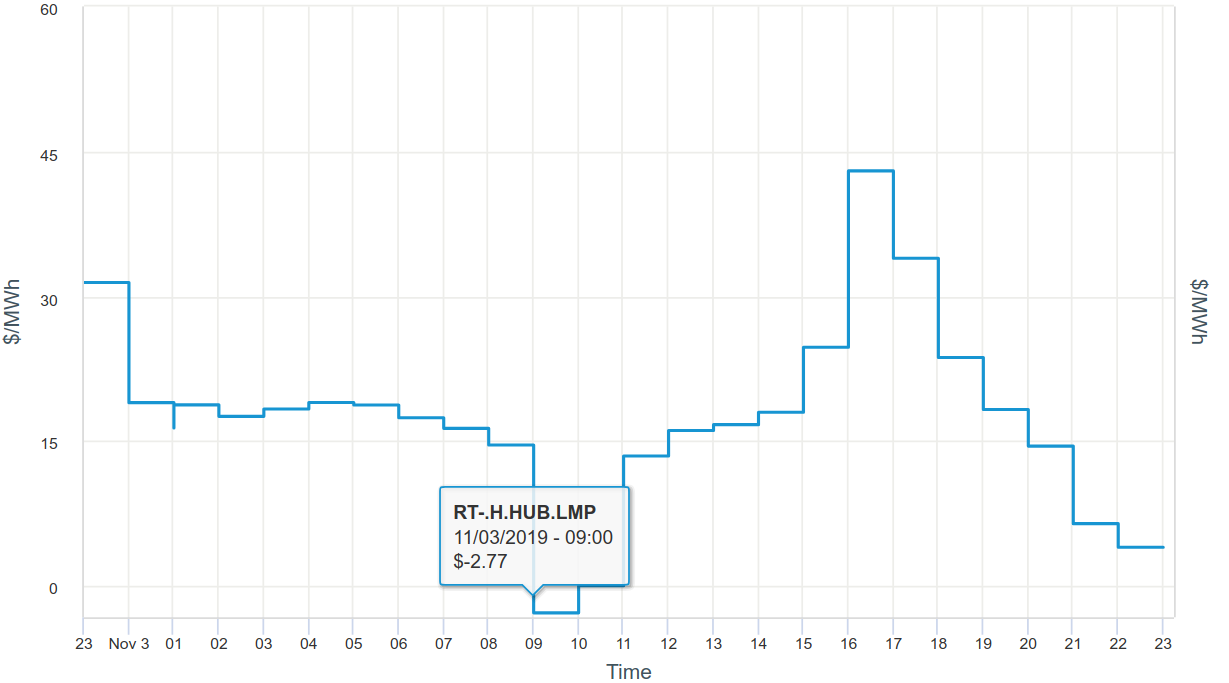
\includegraphics[width=\textwidth]{./images/ne_one_day_price.png}
		\vspace{-6mm}
	\caption{ISO New England hourly electricity price; November 3, 2019 
	from 00:00AM to 11:00PM (Source: https://www.iso-ne.com/).}
\end{figure}  
\end{textblock*}
\end{frame}

\begin{frame}
\frametitle{Nuclear Power Plants as a base-load vs load-following}
\begin{textblock*}{12cm}(0.4cm,1.5cm) % {block width} (coords)
\begin{overlayarea}{\linewidth}{20\baselineskip}
	\begin{block}{Historically used as base-load source of electricity}<1->
		\begin{enumerate}
			\item Usually simpler and more efficient
			\item Nuclear fraction in total power generation was small
			\item Maneuvering capabilities limited to frequency regulation
		\end{enumerate}
	\end{block}
	\begin{block}{Motivation for load-following with nuclear power}<2->
	\begin{enumerate}
		\item The share of nuclear power in total generation became large 
		(75\% in France)
		\item Large-scale deployment of intermittent renewables (up to 40\% in 
		California)
		\item Nuclear power is \textbf{carbon-free, non-intermittent}
	\end{enumerate}
	\end{block}
	\begin{block}{Physical effects in \gls{LWR} limiting the maneuvering 
	capabilities 
		\cite{lokhov_technical_2011}}<3->
	\begin{enumerate}
		\item<3-> Moderator effect (primary coolant temperature change)
		\item<3-> Doppler effect (fuel temperature change)
		\item<4-> Fuel burnup (low excess of reactivity at the end-of-cycle 
		(EOC))
		\item<5-> \textbf{Xenon-135 poisoning (iodine pit)}
	\end{enumerate}
\end{block}
\end{overlayarea}
\end{textblock*}
\end{frame}

\begin{frame}
\frametitle{What is Xenon-135 poisoning? \cite{noauthor_nuclear_nodate-1}}
\animategraphics[loop,controls,width=1.07\linewidth]{0.5}{./images/anime/xe_pois-}{0}{11}
\end{frame}

\subsection{Molten Salt Reactors}

%\begin{frame}
%\frametitle{Potential Generation IV reactor systems 
%%%\cite{abram_generation-iv_2008}}
%\begin{figure}[t]%
%	\vspace*{-0.1in}
%	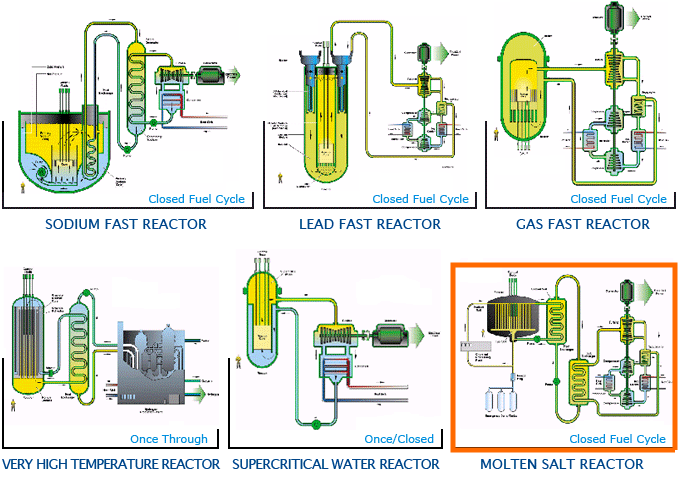
\includegraphics[height=0.7\textwidth]{./images/6_types.png}
%	\caption{\gls{MSR} design}
%\end{figure}            
%\end{frame}

\begin{frame}
\frametitle{MSR (Molten Salt Reactor) types}
\begin{textblock*}{12cm}(0.4cm,1.9cm) % {block width} (coords)
\begin{overlayarea}{\linewidth}{20\baselineskip}
\begin{block}{Stationary Fuel}<1->
	\begin{enumerate}
				\item Graphite block with TRISO fuel, clean salt works as 
				coolant (Fluoride-Salt-Cooled High-Temperature Reactor (FHR))
				\item Plate Fuel: hexagonal fuel assembly is similar in shape 
				to a typical sodium-cooled reactor
				\item Fuel Inside Radial Moderator (FIRM)
	\end{enumerate}
\end{block}

\begin{block}{Mobile Fuel}<2->
	\begin{enumerate}
		\item \textbf{Solid}
			\begin{itemize}
				\item<2-> Mobile solid fuel elements (pebbles) cooled by 
				clean salt (PB-FHR)
			\end{itemize}
			\item<3-> \textbf{Liquid}
			\begin{itemize}
				\item<3-> Without on-site fuel reprocessing facility 
				(TerraPower \glsfirst{MCFR})
				\item<4-> \textbf{With on-site fuel reprocessing} 
				(\glsfirst{TAP} MSR, \glsfirst{MSBR})
			\end{itemize}
	\end{enumerate}
\end{block}
\end{overlayarea}
\end{textblock*}
\end{frame}


%\begin{frame}
%\frametitle{Stationary and Mobile Solid fuel}
%\vspace*{-0.1in}
%\begin{figure}[t]
%	\hspace*{-0.35in}
%	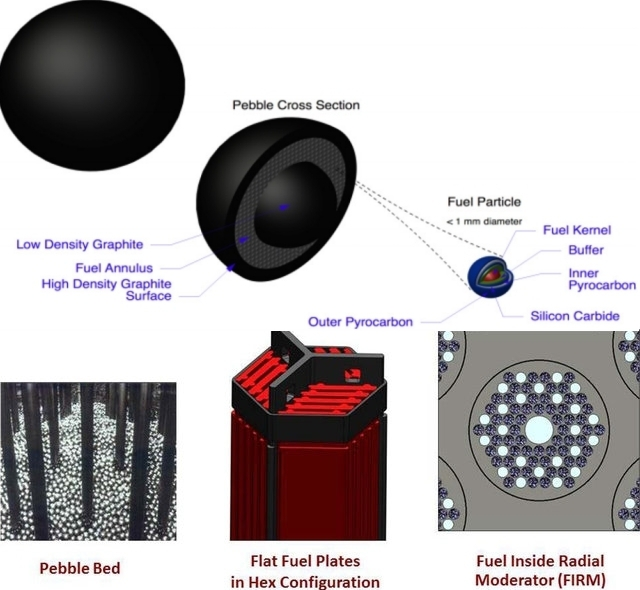
\includegraphics[height=0.63\textwidth]{./images/solid_fuel.jpg}
%	\caption{TRISO fuel particle (top) and FHR fuel designs (bottom) 
%	\cite{forsberg_basis_2016}.} 
%\end{figure}   
%\end{frame}

%\begin{frame}
%\frametitle{Mobile, Non-Circulating, Liquid Fuel}
%\begin{figure}[t]
%\vspace*{-0.1in}
%\hspace*{-0.35in}
%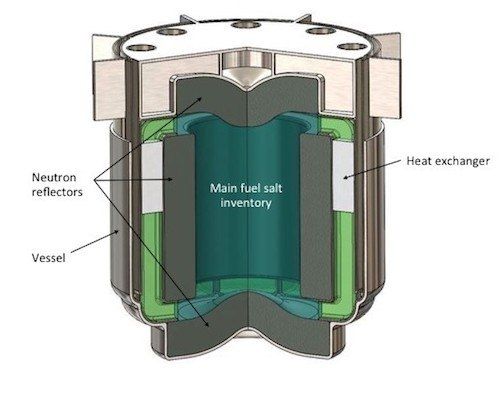
\includegraphics[height=0.6\textwidth]{./images/mcfr-crossection.jpg}
%\caption{The TerraPower MCFR is an example of reactor design with 
%\textbf{liquid, mobile} chloride salt fuel but \textbf{without on-site 
%reprocessing} \cite{doene_southern_2018}.}
%\end{figure}   
%\end{frame}


\begin{frame} % Add another slide with red rectangular around reprocessing system
\frametitle{Mobile, Liquid Fuel with on-site reprocessing facility}
\vspace{-3mm}
\begin{figure}[t]
      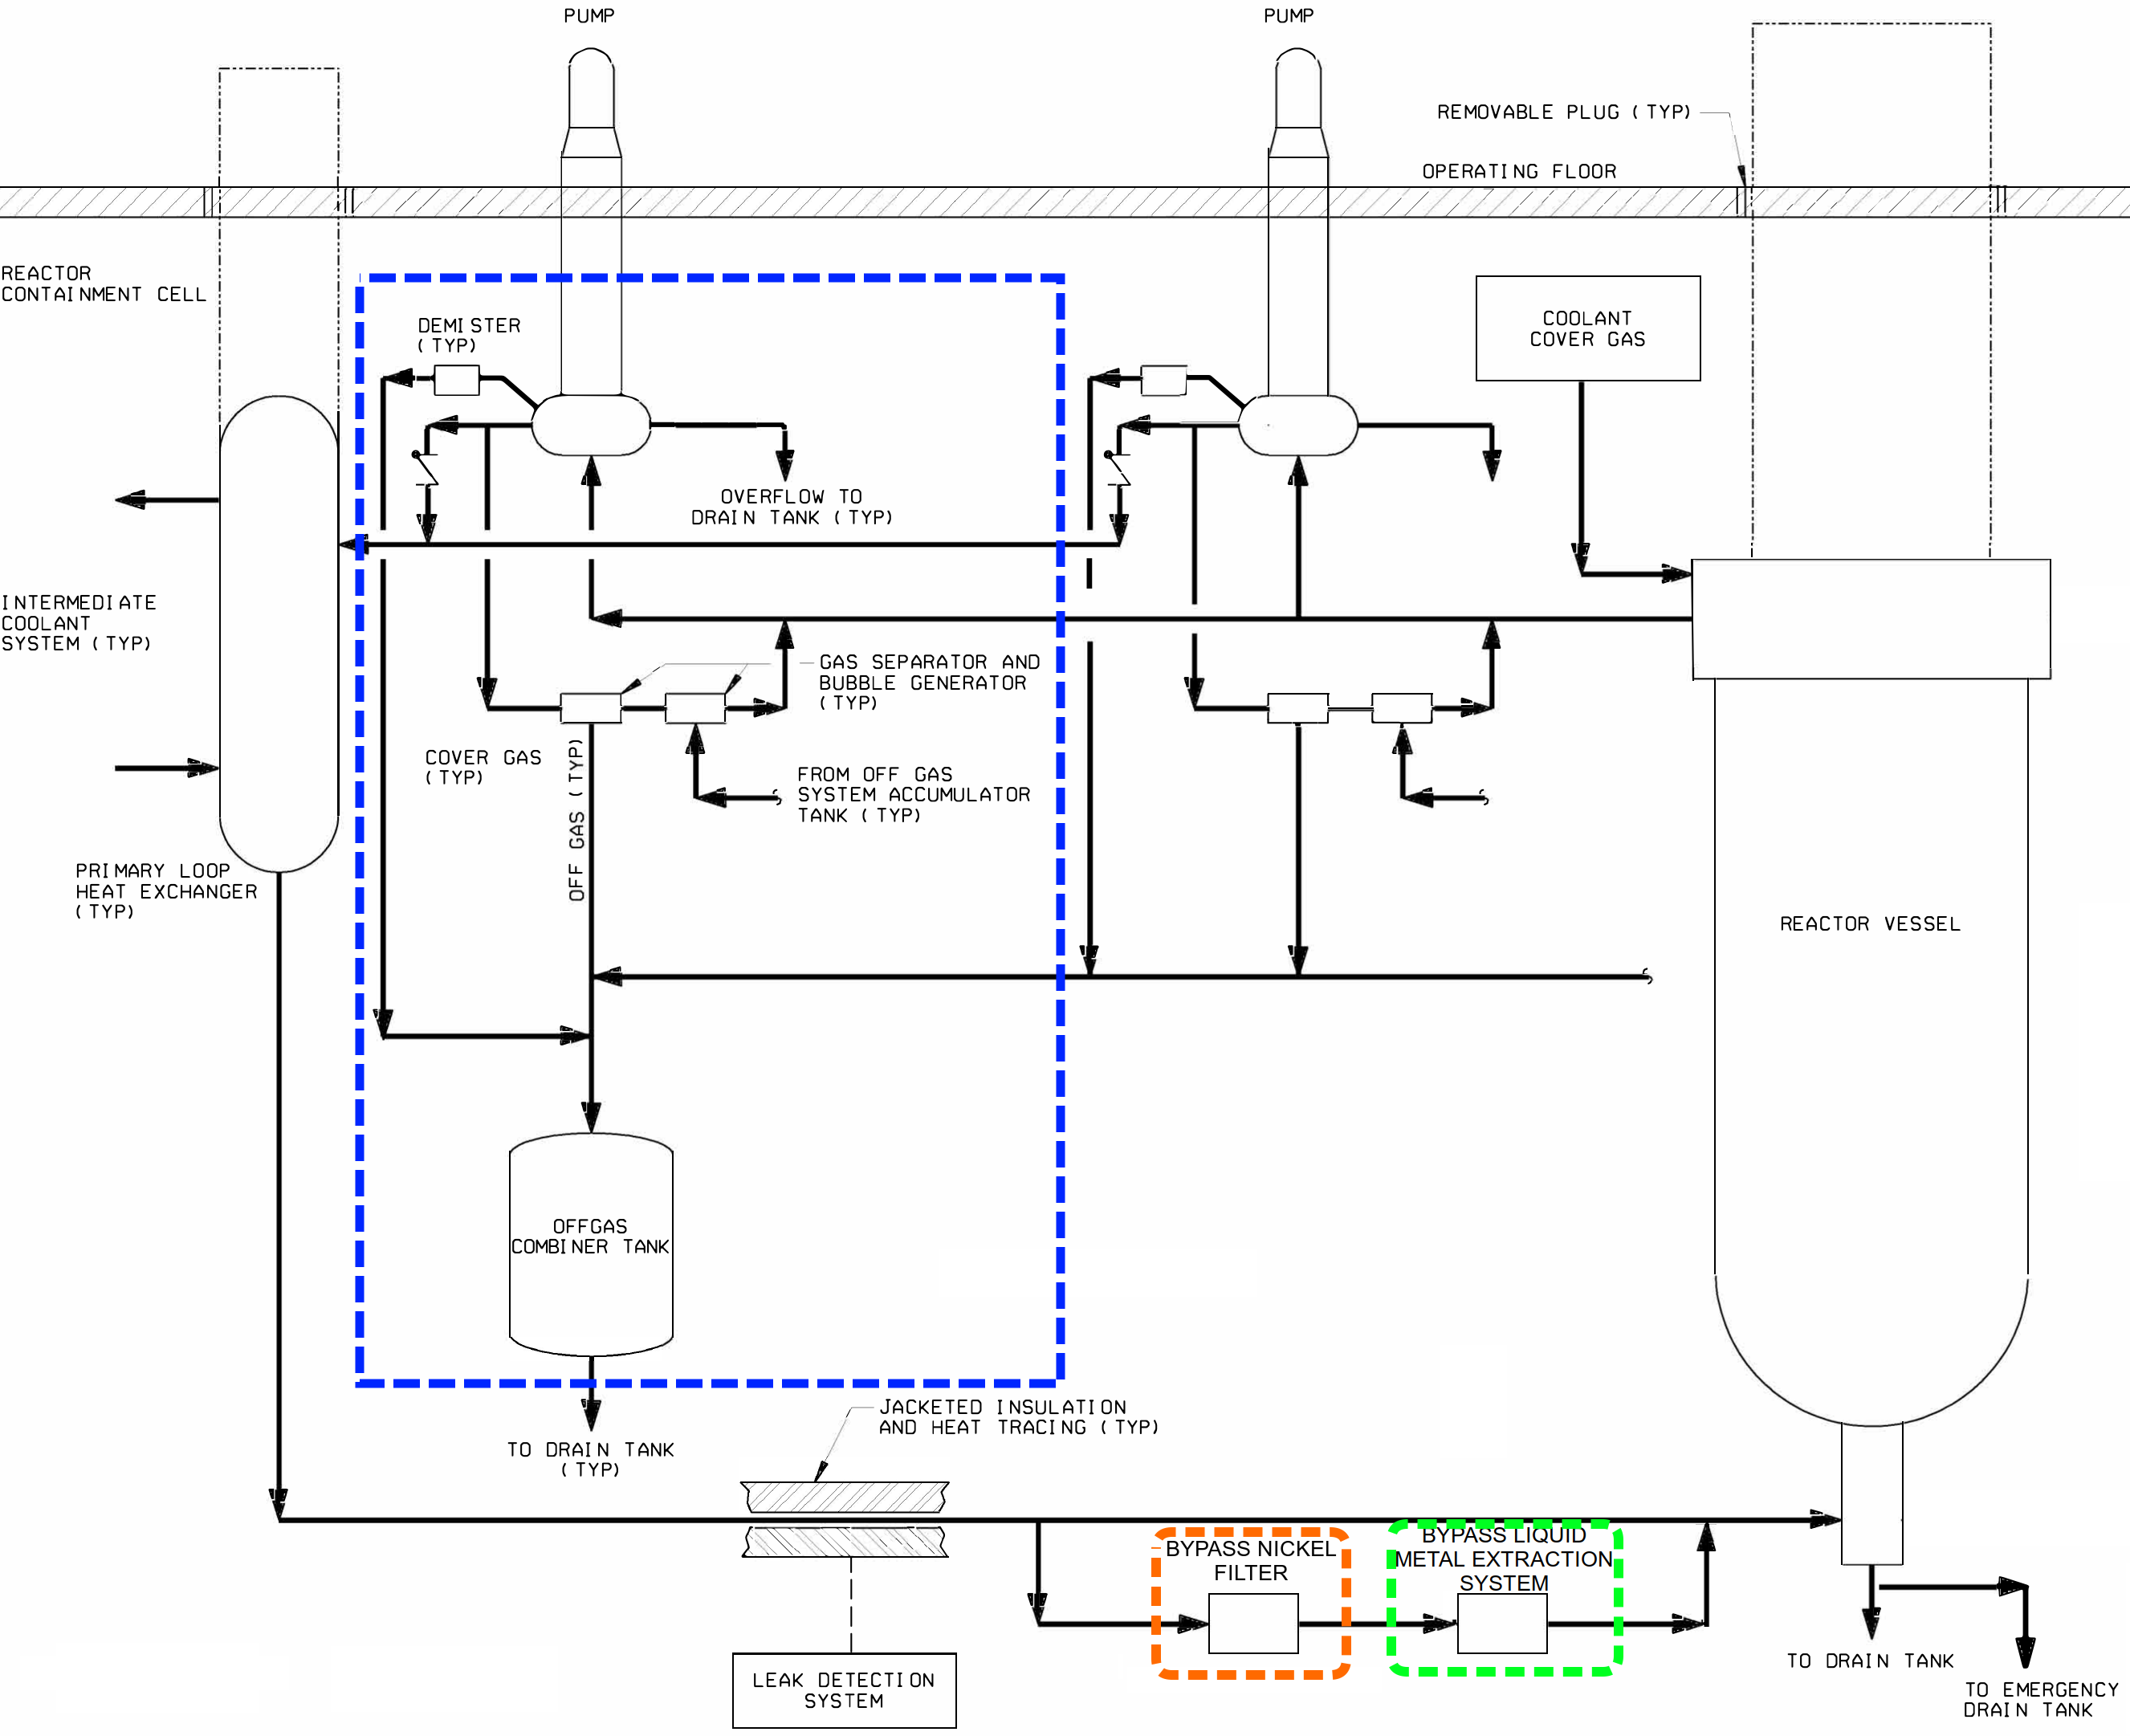
\includegraphics[height=0.67\textwidth]{./images/tap_primary_loop.png}
    \vspace{-2mm}
	\caption{The TAP reactor conceptual schematic (including reprocessing 
	system) \cite{transatomic_power_corporation_technical_2016}.}
\end{figure}   

\end{frame}


\subsection{Motivation}

%\begin{frame}
%\frametitle{Why Molten Salt Reactors with circulating fuel?}
%\begin{block}{Liquid-fueled MSR designs have following \textbf{potential} 
%advantages:}
%	\begin{enumerate}
%		\itemsep1em
%		\item High coolant temperature (600-750$^{\circ}$C) 
%		$\Rightarrow$ potentially high thermal efficiency, process 
%		heat for chemical industry
%		\item Fuel diversity ($^{235}$U, $^{233}$U, Thorium, U/Pu)
%		\item Strong negative fuel temperature feedback 
%		\item Passive safety $\Rightarrow$ fuel drains into tanks 
%		in emergency
%		\item High fuel utilization $\Rightarrow$ reduced spent fuel 
%		generation
%		\item<2> \textbf{On-line (continuous) fuel reprocessing potentially  
%		helps to reduce Xenon-135 poisoning} $\Rightarrow$ more flexible  
%		power maneuvering
%	\end{enumerate}
%\end{block}

%\end{frame}


\subsection{Research objectives}

\begin{frame}
  \frametitle{Research objectives of this work}
     Analyze the TAP MSR neutronic performance during load-following 
     \textbf{at the \glsfirst{BOL}} and \textbf{inactive online fission 
     products removal system}. The neutronics performance for the Middle of 
     Life and End of Life will be different.
  \begin{overlayarea}{\linewidth}{20\baselineskip}
     \begin{block}{Goals of current study}<1->
         \begin{enumerate}
         		\itemsep1em
                \item<1-> Create high-fidelity full-core 3-D model of 
                TAP concept, without any approximations using Serpent 
                \cite{leppanen_serpent_2014}
                \item<2-> Perform fuel salt depletion to study 
                \textbf{$^{135}$Xe/$^{135}$I balance dynamics during 
                load-following}
            	\item<3-> Analyze $k_{eff}$ dynamics during 
            	\textbf{load-following}
                \item<4-> Compare obtained results with well-studied 
                \glsfirst{PWR} behavior
         \end{enumerate}
      \end{block}
  \end{overlayarea}
\end{frame}
